\documentclass{article}
\usepackage[utf8]{inputenc}
\usepackage{graphicx} 
\usepackage{ragged2e}
\usepackage{subfig}
\usepackage[utf8]{inputenc}
\usepackage{float}
\usepackage{amsmath}
\usepackage{tikz-cd}
\usepackage{amssymb}
\usepackage{enumerate}
\usepackage{mathtools}
\usepackage{hyperref}

\newcommand{\norm}[1]{\left\lVert#1\right\rVert}

\title{Actividades propuestas}


\author{Carlos A. Toro, Lucas H. Quiceno, Victor M. Oviedo}
\date{Agosto 2021}

\begin{document}

\maketitle

\section{Instrucciones de uso}

El usuario se encontrará con tres barras laterales, como se muestra en la Figura 2, donde podrá variar los siguientes parámetros:
\begin{figure}[h]
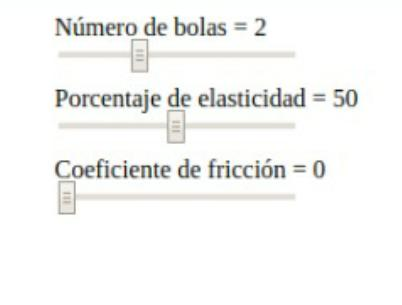
\includegraphics[width=\linewidth]{lab1.jpeg}
\caption{Primer panel de simulación.}
\end{figure}

\begin{itemize}
     \item Número de bolas: Se puede escoger, variando la primera barra horizontal, entre 1 bola y 6 bolas, en el siguiente orden. 
    \begin{itemize} \item Amarilla \item Roja \item Azúl \item Morada \item Naranja \item Rosada
    \end{itemize}
     Este es el orden en el que aparecen las bolas, si el usuario ingresa, digamos tres bolas, le aparecen en los colores de las tres primeras de la lista anterior. 
    
   
    \item En la segunda barra horizontal se puede variar el porcentaje de elasticidad que le permite al usuario ver colisiones elásticas o inelásticas de acuerdo al coeficiente que escoja.
    \item El coeficiente de proporcionalidad $b$: Este coeficiente es el responsable de la fricción con el medio y con la mesa, el coeficiente puede tomar valores entre 0 y 1 y lo puede escoger al variar la barra horizontal.  
    
    \begin{figure}[h]
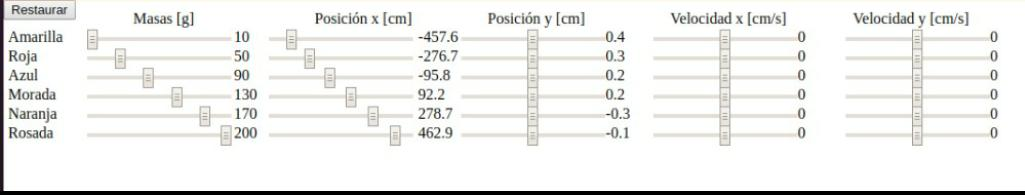
\includegraphics[width=\linewidth]{lab2.jpeg}
\caption{Segundo panel de simulación.}
\end{figure}

   
    \item En la parte inferior se encontrará con seis barras que le permiten variar los parámetro de las bolas, como su masa y al variar la masa, se varía el radio por la relación $M = \rho V $ donde $M$ es la masa de cada bola, $\rho$ es su densidad que depente del medio, para nuestro caso $\rho = 6\ g/cm^{3}$ y el volumen es $V = \frac{4\pi R^{3}}{3}$, con estas consideraciones, la masa de cada bola se puede escribir en función del radio como $M = \rho \frac{4\pi R^{3}}{3}$
    \item En la parte inferior, Figura 3, se puede encontrar al frente del color de cada bola las barras donde puede variar los parámetros, cómo velocidades iniciales en $x$ y en $y$, posición iniciales en $x$ y en $y$, ajuste estos parámetros de acuerdo a su gusto.
     \begin{figure}[h]
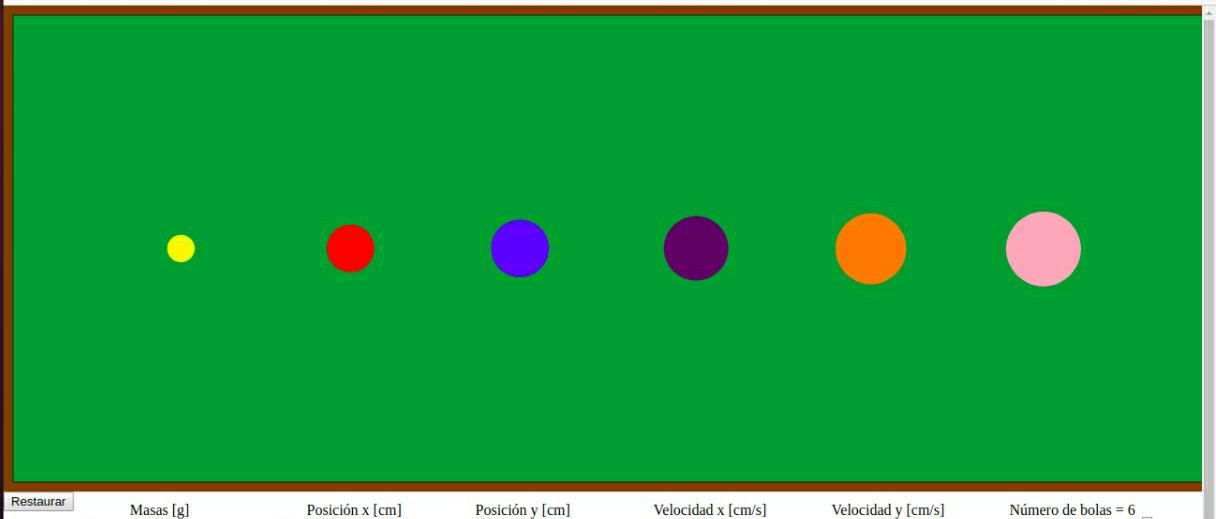
\includegraphics[width=\linewidth]{lab3.jpeg}
\caption{Segundo panel de simulación.}
\end{figure}

    \item Finalmente, al seguir todos los pasos anteriores, se econtrará un panorama como en la Figura 4. Solo resta que le de en el botón restaurar y con eso se dará inicio a la simulación.
\end{itemize}
Se encontrará los datos que el programa le arroja para para velocidades finales, energía cinética inicial y final, momento lineal inicial y final, de acuerdo a los parámetros que usted ingresa al principio de la simulación. Usted puede graficar esos datos o mirar el comportamiento de las cantidades físicas, puede observar la conservación del momento y de la energía de acuerdo a la cantidad que escoja.


\section{Actividades}
\begin{itemize} 
\item Las fuerzas disipativas, como la fricción, están presentes en los fenómenos físicos con los que nos encontramos en la vida cotidiana. Para que el usuario vea los efectos de la fricción en la simulación se propone que ponga una única bola con velocidad máxima en $x$ y en $y$ y note como cambia el tiempo que demora la bola en quedarse quieta a medida que se varía el factor que determina la fricción.
\item Para estudiar la transferencia de momento se propone simular tres bolas con la mínima masa, poner una de ellas en el origen, es decir, en la posición $(0,0)$, justo al lado de esta poner otra en la posición $(0,20)$ y para la tercera bola se pondrá 0 en el eje vertical y la posición mínima en el eje horizontal. Las primeras dos bolas estarán inicialmente quietas, mientras que a la tercera se le pondrá velocidad máxima en el eje horizontal y 0 en el vertical. Finalmente seleccionamos choque completamente elástico y 0 fricción. Con ello queremos simular un escenario donde hay transferencia de momento lineal entre los tres objetos pero únicamente hay una bola en movimiento en cada momento de la simulación. 
\item Graficar como evoluciona la energía cinética del sistema de seis bolas de billar para diferentes valores del coeficiente de fricción y del porcentaje de elásticidad. 
\item Finalmente se le propone al usuario volver al escenario donde están las seis bolas, variar masa a su gusto, así como velocidades iniciales y posiciones, pero ahora que experimente con el porcentaje de elasticidad y pueda ver como el sistema va perdiendo energía a medida que se van presentando colisiones. Se recomienda que las velocidades en el eje vertical sean diferentes de 0 para aprovechar el carácter bidimensional de la simulación.
\end{itemize}
\section{Referencias}
[1] Young, Hugo D. y Freedman, Roger A. Física Universitaria Vol. I, Decimosegunda edición, PEARSON EDUCACÍON, 2009.

[2] https://www.sjsu.edu/faculty/watkins/collision.htm


\end{document}





\end{document}
